% Copyright 2004 by Till Tantau <tantau@users.sourceforge.net>.
%
% In principle, this file can be redistributed and/or modified under
% the terms of the GNU Public License, version 2.
%
% However, this file is supposed to be a template to be modified
% for your own needs. For this reason, if you use this file as a
% template and not specifically distribute it as part of a another
% package/program, I grant the extra permission to freely copy and
% modify this file as you see fit and even to delete this copyright
% notice. 

\documentclass{beamer}
\usepackage{boondox-cal}
\usepackage{tikz}
\usetikzlibrary{bayesnet}
\usepackage{kotex}
\usepackage{amsfonts}
\usepackage{subcaption}
\captionsetup{compatibility=false}
\usepackage{amssymb}
\newcommand{\E}{\mathbb{E}}
\usepackage{amsthm}
\usepackage{latexsym,amsmath}
\usepackage{graphicx}
\usepackage{pgfplots}
\usepackage{afterpage}
\usepackage[ ]{algorithm2e}
\usepackage{bm}
\newcommand{\R}{\mathbb{R}}
\DeclareMathOperator*{\argmin}{arg\,min}
% There are many different themes available for Beamer. A comprehensive
% list with examples is given here:
% http://deic.uab.es/~iblanes/beamer_gallery/index_by_theme.html
% You can uncomment the themes below if you would like to use a different
% one:
%\usetheme{AnnArbor}
%\usetheme{Antibes}
%\usetheme{Bergen}
%\usetheme{Berkeley}
%\usetheme{Berlin}
%\usetheme{Boadilla}
%\usetheme{boxes}
%\usetheme{CambridgeUS}
%\usetheme{Copenhagen}
%\usetheme{Darmstadt}
%\usetheme{default}
%\usetheme{Frankfurt}
%\usetheme{Goettingen}
%\usetheme{Hannover}
%\usetheme{Ilmenau}
%\usetheme{JuanLesPins}
%\usetheme{Luebeck}
\usetheme{Madrid}
%\usetheme{Malmoe}
%\usetheme{Marburg}
%\usetheme{Montpellier}
%\usetheme{PaloAlto}
%\usetheme{Pittsburgh}
%\usetheme{Rochester}
%\usetheme{Singapore}
%\usetheme{Szeged}
%\usetheme{Warsaw}

\title{Density Ratio Estimators in Variational Bayesian Machine Learning}

% A subtitle is optional and this may be deleted
%\subtitle{Optional Subtitle}

\author{Lammy}
% - Give the names in the same order as the appear in the paper.
% - Use the \inst{?} command only if the authors have different
%   affiliation.

\institute[UNSW] % (optional, but mostly needed)
{
  Department of Mathematics and Statistics\\
  UNSW
  }
% - Use the \inst command only if there are several affiliations.
% - Keep it simple, no one is interested in your street address.

\date{Statistics Honours, 2018}
% - Either use conference name or its abbreviation.
% - Not really informative to the audience, more for people (including
%   yourself) who are reading the slides online

\subject{Statistics}
% This is only inserted into the PDF information catalog. Can be left
% out. 

% If you have a file called "university-logo-filename.xxx", where xxx
% is a graphic format that can be processed by latex or pdflatex,
% resp., then you can add a logo as follows:

% \pgfdeclareimage[height=0.5cm]{university-logo}{university-logo-filename}
% \logo{\pgfuseimage{university-logo}}

% Delete this, if you do not want the table of contents to pop up at
% the beginning of each subsection:
%\AtBeginSection[]
%{
%  \begin{frame}<beamer>{Outline}
%    \tableofcontents[currentsection,currentsubsection]
%  \end{frame}
%}

% Let's get started
\begin{document}

\begin{frame}
  \titlepage
\end{frame}

\begin{frame}{Outline}
  \tableofcontents
  % You might wish to add the option [pausesections]
\end{frame}

% Section and subsections will appear in the presentation overview
% and table of contents.
\section{Background Info}

\subsection{Neural Networks}

\begin{frame}{Neural Networks}{Overall Structure}
  \begin{itemize}
  \item {
    Mathematical model based off human brain.
  }
  \item {
  	Objective is to approximate a function $f^*$ using mapping with parameters $\bm{\Theta}$: $\textbf{f}_{\bm{\Theta}}(\bm{x})$.  
  }
  \item {
  	Universal Approximation Theorem states a neural network can approximate (almost) any function if it is complex enough.
  }
  \item {
    Consists of layers of nodes:
  }
  \end{itemize}
  \begin{figure}[h]
  \resizebox{.5\linewidth}{!}{
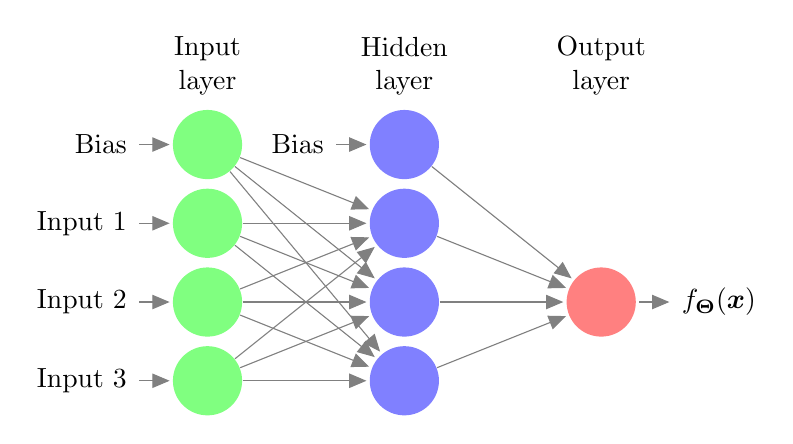
\begin{tikzpicture}[shorten >=1pt,->,draw=black!50, node distance=2.5cm]
    \tikzstyle{every pin edge}=[<-,shorten <=1pt]
    \tikzstyle{neuron}=[circle,fill=black!25,minimum size=25pt,inner sep=0pt]
    \tikzstyle{input neuron}=[neuron, fill=green!50];
    \tikzstyle{output neuron}=[neuron, fill=red!50];
    \tikzstyle{hidden neuron}=[neuron, fill=blue!50];
    \tikzstyle{annot} = [text width=4em, text centered]
    
	\node[input neuron, pin=left:Bias] (I-0) at (0,0) {};
    % Draw the input layer nodes
    \foreach \name / \y in {1,...,3}
    % This is the same as writing \foreach \name / \y in {1/1,2/2,3/3,4/4}
        \node[input neuron, pin=left:Input \y] (I-\name) at (0,-\y) {};

 \path[yshift=0cm]
            node[hidden neuron, pin=left:Bias] (H-0) at (2.5cm,0) {};
    % Draw the hidden layer nodes
    \foreach \name / \y in {1,...,3}
        \path[yshift=0cm]
            node[hidden neuron] (H-\name) at (2.5cm,-\y) {};

    % Draw the output layer node
	\path[yshift=1cm]    
    node[output neuron,pin={[pin edge={->}]right:$f_{\bm{\Theta}}(\bm{x})$}, right of=H-2] (O) {};

    % Connect every node in the input layer with every node in the
    % hidden layer.
    \foreach \source in {0,...,3}
        \foreach \dest in {1,...,3}
            \path (I-\source) edge (H-\dest);

    % Connect every node in the hidden layer with the output layer
    \foreach \source in {0,...,3}
        \path (H-\source) edge (O);

    % Annotate the layers
    \node[annot,above of=H-0, node distance=1cm] (hl) {Hidden layer};
    \node[annot,left of=hl] {Input layer};
    \node[annot,right of=hl] {Output layer};
\end{tikzpicture}
}
\end{figure}

\end{frame}
\begin{frame}{Neural Networks}{Individual Node Structure}
\begin{itemize}
\item Each node is a generalised linear model of preceding layer output.
\item Weights $\theta$ are randomly initialised.
\item Bias $x_0=1$ has role of intercept term in typical regression.
\item $g(x)$ is activation function, e.g. ReLU is $g(x)=\max\{0,x\}$ in $[0,\infty)$, Sigmoid is $g(x)=(1+\exp(-x))^{-1}$ in $(0,1)$.
\begin{figure}[h]
  \resizebox{.4\linewidth}{!}{
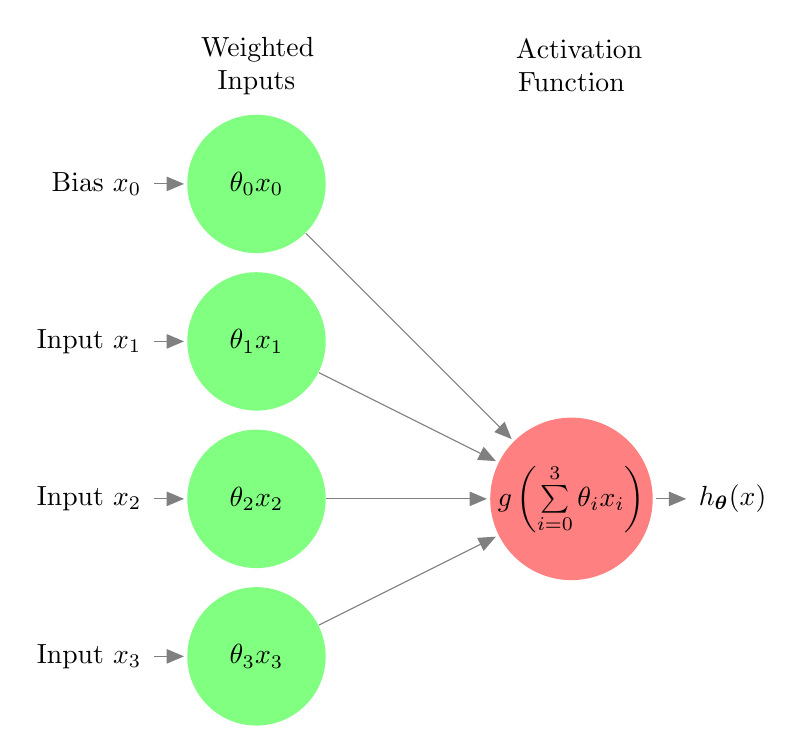
\begin{tikzpicture}[shorten >=1pt,->,draw=black!50, node distance=2.5cm]
    \tikzstyle{every pin edge}=[<-,shorten <=1pt]
    \tikzstyle{neuron}=[circle,fill=black!25,minimum size=50pt,inner sep=0pt]
    \tikzstyle{input neuron}=[neuron, fill=green!50];
    \tikzstyle{output neuron}=[neuron, fill=red!50];
    \tikzstyle{hidden neuron}=[neuron, fill=blue!50];
    \tikzstyle{annot} = [text width=4em, text centered]

    % Draw the input layer nodes
 %   \foreach \name / \y in {0,...,3}
    % This is the same as writing \foreach \name / \y in {1/1,2/2,3/3,4/4}
        \node[input neuron, pin=left:Bias $x_0$] (I-0) at (0,-0) {$\theta_0 x_0$};
	\foreach \name / \y in {1,...,3}
    % This is the same as writing \foreach \name / \y in {1/1,2/2,3/3,4/4}
        \node[input neuron, pin=left:Input $x_{\y}$] (I-\name) at (0,-2*\y) {$\theta_{\y}x_\y$};
    % Draw the hidden layer nodes
    %\foreach \name / \y in {1,...,5}
     %   \path[yshift=0.5cm]
      %      node[hidden neuron] (H-\name) at (\layersep,-\y cm) {};

    % Draw the output layer node
    \node[output neuron,pin={[pin edge={->}]right:$h_{\bm{\theta}}(x)$}, right of=I-2, node distance=4cm] (O) {$g\left(\sum\limits^3_{i=0}\theta_ix_i\right)$};

    % Connect every node in the input layer with every node in the
    % hidden layer.
   % \foreach \source in {1,...,4}
    %    \foreach \dest in {1,...,5}
     %       \path (I-\source) edge (H-\dest);

    % Connect every node in the hidden layer with the output layer
    \foreach \source in {0,...,3}
        \path (I-\source) edge (O);

    % Annotate the layers
%    \node[annot,above of=H-1, node distance=1cm] (hl) {Hidden layer};
    \node[annot,above of=I-0, node distance=1.5cm](il) {Weighted Inputs};
    \node[annot,right of=il, node distance=4cm] {Activation Function};
\end{tikzpicture}
}
\end{figure}

\end{itemize}
\end{frame}
\begin{frame}{Neural Networks}{Training}
\begin{itemize}
\item Weights and biases trained such that (ideally convex) loss function is minimized e.g. Mean Squared Error: $\min_\Theta \frac{1}{2}||\bm{y}-\bm{f}_\Theta(\bm{x})||^2_2$.
\item Back-propagation finds partial derivatives of loss function with respect to weights.
\item Gradient descent uses these partial derivatives to optimize network.
\end{itemize}
\end{frame}
\subsection{(Amortized) Variational Inference}

% You can reveal the parts of a slide one at a time
% with the \pause command:
\begin{frame}{(Amortized) Variational Inference}{Bayesian Inference}
  \begin{itemize}
  \item {
    Fundamental problem in Bayesian computation is to estimate posterior densities $p(z|x)$.
    %\pause % The slide will pause after showing the first item
  }
  \begin{equation*}
p(z|x)=\frac{p(z,x)}{p(x)}= \frac{p(z)p(x|z)}{\int_\mathcal{z}p(z,x)dz}
\end{equation*}
  \item {   
    Problems arise when $\int_\mathcal{z}p(z,x)dz$ is computationally intractable.
  }
  % You can also specify when the content should appear
  % by using <n->:
  \item {
    Typical MCMC methods are slow with large datasets or high dimensional data.
  }
  % or you can use the \uncover command to reveal general
  % content (not just \items):
  \item {
    Variational Inference is a solution.
  }
  \end{itemize}
\end{frame}
\begin{frame}{(Amortized) Variational Inference}{Introduction}
\begin{itemize}
\item Amortized variational inference approximates $p(z|x)$ with a different distribution $q_\phi(z|x)$.
\item $q_\phi(z|x)$ is a neural network with parameters $\phi$ that takes in data $x$ and random noise $\epsilon\sim \pi(\epsilon)$ and outputs samples $z\sim q_\phi(z|x)$.
\item Typically $\pi(\epsilon)=\mathcal{N}(0,I_{n\times n})$.
\begin{figure}[h]
  \centering
  \tikz{ %
    \node[latent] (x) {$x$} ; %
    \node[det, right=of x] (q) {$q_\phi(z|x)$} ; %
    \node[latent, right=of q] (qout) {$z$} ;
    \node [latent, above=of x] (eps) {$\epsilon$} ;
    \edge {x} {q} ; %
    \edge {eps} {q} ;
    \edge {q} {qout} ;
  }
\end{figure}
\end{itemize}
\end{frame}
\begin{frame}{(Amortized) Variational Inference}{Network Training}
\begin{itemize}
\item Minimize the \textbf{n}egative of the \textbf{e}vidence \textbf{l}ower \textbf{bo}und $NELBO(q)$:
\[\min_\phi NELBO(q)=-\mathbb{E}_{q_\phi(z|x)q^*(x)}[\log p(x|z)]+\mathbb{E}_{q^*(x)}[KL(q_\phi(z|x)||p(z))].\]
\item This is the same as minimizing the reverse KL divergence between the two distributions:
\[\E_{q^*(x)}[KL(q(z|x)||p(z|x))]=\mathbb{E}_{q^*(x)q(z|x)}\left[\log \left(\frac{q(z|x)}{p(z|x)}\right)\right]\].
\item Taking expectation with respect to dataset distribution $q^*(x)$ allows model to work for different data points.
\end{itemize}
\end{frame}
\begin{frame}{(Amortized) Variational Inference}{Prior-Contrastive}
\[\min_\phi \underbrace{-\mathbb{E}_{q_\phi(z|x)q^*(x)}[\log p(x|z)]}_\text{Likelihood}+\underbrace{\mathbb{E}_{q^*(x)}[KL(q_\phi(z|x)||p(z))]}_\text{Log Density Ratio}.\]
\begin{itemize}
\item $q_\phi(z|x)$ is a neural network so extremely difficult to evaluate density function but easy to draw samples, we therefore say that it is \textbf{implicit}.
\item Use density ratio estimation to evaluate $\frac{q_\phi(z|x)}{p(z)}$ in $KL(q_\phi(z|x)||p(z))$.
\item The prior $p(z)$ can also be implicit.
\item We call this the ``prior-contrastive" formulation.
\end{itemize}
\end{frame}
\begin{frame}{(Amortized) Variational Inference}{Joint-Contrastive}
\begin{itemize}
\item If the likelihood $p(x|z)$ is implicit, then our optimization problem is \[\min_\phi KL(q(z,x)||p(z,x))=\E_{q^*(x)q_\phi(z|x)}\log \frac{q^*(x)q_\phi(z|x)}{p(z)p(x|z)}.\]
\item Use density ratio estimation to evaluate $\frac{q(z,x)}{p(z,x)}$.
\item For consistency, $NELBO(q)= KL(q(z,x)||p(z,x))$.
\item We call this the ``joint-contrastive" formulation.
\end{itemize}
\end{frame}
%\begin{frame}{(Amortized) Variational Inference}{Autoencoders}
%\begin{itemize}
%\item An autoencoder consists of an encoder $q_\phi(z|x)$ that `compresses' data $x$ into lower dimensional latent $z$, and a decoder $p_\theta(x|z)$ that generates data $x$ from $z$.
%\item This is the same as our Bayesian inference problem except the likelihood is a neural network parametrised with $\theta$.
%\item To generate new data, sample $z\sim p(z)$ and pass through decoder.
%\item We typically know $p_\theta(x|z)$ in explicit form e.g. if $x$ is grey-scale image data, then $p_\theta(x|z)$ is a Bernoulli distribution with parameters given by sigmoid output of the neural network.
%\item Therefore have optimization problem $\min_{\theta, \phi} -\mathbb{E}_{q_\phi(z|x)q^*(x)}[\log p_\theta(x|z)]+\mathbb{E}_{q^*(x)}[KL(q_\phi(z|x)||p(z))].$
%\item If $p_\theta(x|z)$ is implicit then we have the optimization problems $\min_\phi KL(q(z,x)||p(z,x))$ and $\min_\theta KL(p(z,x)||q(z,x))$.
%\end{itemize}
%\end{frame}
\subsection{Density Ratio Estimation}

% You can reveal the parts of a slide one at a time
% with the \pause command:
\begin{frame}{Density Ratio Estimation}{Class Probability Estimation}
We want to estimate $\frac{q(u)}{p(u)}$.
  \begin{enumerate}
  \item {
    Define discriminator function that finds probability that a sample $u$ came from $q(u)$: $D_\alpha(u)\simeq P(u\sim q(u))$, so that $\frac{q(u)}{p(u)}\simeq \frac{D_\alpha(u)}{1-D_\alpha(u)}$.
  }
  \item $D_\alpha(u)$ is neural network parametrised by $\alpha$, sigmoid activation function used for output layer
  % or you can use the \uncover command to reveal general
  % content (not just \items):
  \item {
    Train discriminator with Bernoulli loss: $\min_\alpha -\mathbb{E}_{q(u)}[\log D_\alpha(u)]-\mathbb{E}_{p(u)}[\log(1-D_\alpha(u))]$.
  }
  \item Optimal discriminator is $D^*_\alpha(u)=\frac{q(u)}{q(u)+p(u)}$.
  \end{enumerate}
\end{frame}
\begin{frame}{Density Ratio Estimation}{Class Probability Estimation}
Prior-Contrastive Application:
\[\min_\alpha -\mathbb{E}_{q^*(x)q_\phi(z|x)}[\log D_\alpha(z,x)]-\mathbb{E}_{q^*(x)p_\theta(z)}[\log (1-D_\alpha(z,x))]\]
\[\min_\phi \underbrace{-\mathbb{E}_{q^*(x)q_\phi(z|x)}[\log p(x|z)]}_\text{Likelihood}+\underbrace{\mathbb{E}_{q^*(x)q_\phi(z|x)}\left[\log \frac{D_\alpha(z,x)}{1-D_\alpha(z,x)}\right]}_\text{Log Density Ratio}\]
Joint-Contrastive Application:
\[\min_\alpha -\mathbb{E}_{q^*(x)q_\phi(z|x)}[\log D_\alpha(z,x)]-\mathbb{E}_{p(z)p(x|z)}[\log (1-D_\alpha(z,x))]\]
\[\min_\phi \mathbb{E}_{q^*(x)q_\phi(z|x)}\log\frac{D_\alpha(z,x)}{1-D_\alpha(z,x)}\]
Program alternates between several optimisation steps of discriminator and one optimisation step of posterior.
\end{frame}
\begin{frame}{Density Ratio Estimation}{Divergence Minimisation}
\begin{theorem}
If $f$ is a convex function with derivative $f'$ and convex conjugate $f^*$, and $\mathcal{R}$ is a class of functions with codomains equal to the domain of $f'$, then we have the lower bound for the f-divergence between distributions $p(u)$ and $q(u)$:
\[D_f [p(u)||q(u)]\geq \sup_{r\in \mathcal{R}} \{\mathbb{E}_{q(u)}[f'(r(u))]-\mathbb{E}_{p(u)}[f^*(f'(r(u)))]\},\]
with equality when $r(u)=q(u)/p(u)$.
\end{theorem}
For the reverse KL divergence, $f(u)=u\log u$ so we have
\[KL[q(u)||p(u)]\geq \sup_{r\in \mathcal{R}}\{\mathbb{E}_{q(u)}[1+\log r(u)]-\mathbb{E}_{p(u)}[r(u)]\}\]

\end{frame}
\begin{frame}{Density Ratio Estimation}{Divergence Minimisation}
\begin{itemize}
\item Let our ratio estimator be a neural network parametrised by $\alpha$: $r_\alpha(u)\simeq \frac{q(u)}{p(u)}$.
\item Maximise the lower bound w.r.t. $\alpha$ until equality, which is when $r_\alpha(u)=\frac{q(u)}{p(u)}$. The optimisation problem for this is
\[\min_\alpha -\mathbb{E}_{q(u)}[\log r_\alpha(u)]+\mathbb{E}_{p(u)}[r_\alpha(u)].\]
\item Obviously our optimal ratio estimator is $r^*_\alpha(u)=\frac{q(u)}{p(u)}$.
\end{itemize}
\end{frame}
\begin{frame}{Density Ratio Estimation}{Divergence Minimisation}
Prior-Contrastive Application:
\[\min_\alpha -\E_{q^*(x)q_\phi(z|x)}[\log r_\alpha(z,x)]+\E_{q^*(x)p(z)}[r_\alpha (z,x)]\]
\[\min_\phi \underbrace{-\mathbb{E}_{q^*(x)q_\phi(z|x)}\left[\log p(x|z)\right]}_\text{Likelihood}+\underbrace{E_{q^*(x)q_\phi (z|x)}[\log r_\alpha(z,x)]}_\text{Log Density Ratio}\]
Joint-Contrastive Application:
\[\min_\alpha-\E_{q^*(x)q_\phi(z|x)}[\log r_\alpha(z,x)]+\E_{p(z)p(x|z)}[r_\alpha(z,x)]\]
\[\min_\phi \mathbb{E}_{q^*(x)q_\phi(z|x)}[\log r_\alpha(z,x)]\]
\end{frame}
\begin{frame}{Density Ratio Estimation}{Algorithm Generalisation}
\begin{itemize}
\item Actually, $f(u)=u\log u-(u+1)\log (u+1)$ and $D(u)=\frac{r(u)}{r(u)+1}$ leads to class probability estimation equations.
\item The upper bound f-divergence is $2JS(p(u)\|q(u))-\log 4$, we call this the GAN divergence.
\item To formulate optimisation problems for density ratio estimation, choose either reverse KL or GAN f-divergence upper bound and estimator parametrisation:
\begin{itemize}
\item Class Probability Estimator $D_\alpha(u)\simeq \frac{q(u)}{q(u)+p(u)}$
\item Direct Ratio Estimator $r_\alpha(u)\simeq \frac{q(u)}{p(u)}$
\item Direct Log Ratio Estimator $T_\alpha(u)\simeq\log \frac{q(u)}{p(u)}$.
\end{itemize}
\end{itemize}
\end{frame}
\section{Activation Function Experiment}
\begin{frame}{Activation Function Experiment}{Experiment Outline}
\[p(z_1,z_2)\sim \mathcal{N} (0,\sigma^2 I_{2\times 2})\]
\[p(x|\bm{z})\sim EXP(3+\max(0,z_1)^3+\max(0,z_2)^3)\]
\begin{figure}[h]
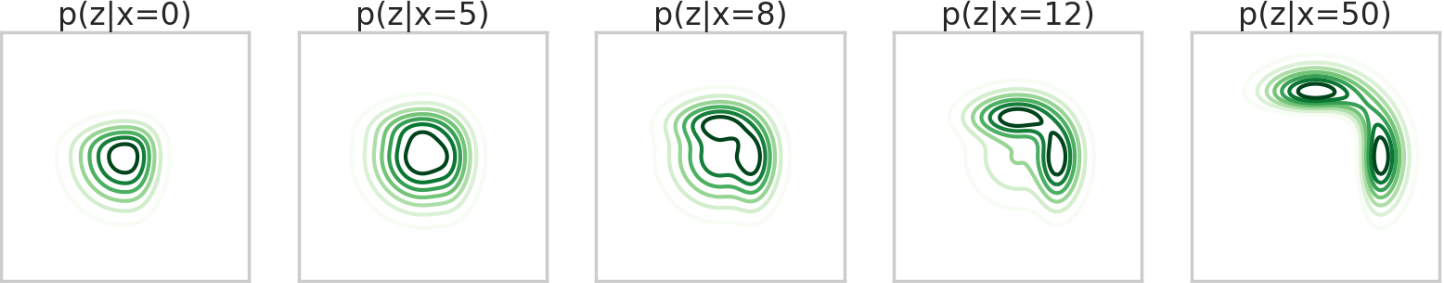
\includegraphics[width=\textwidth]{sprinklertrue.png}
\end{figure}
\begin{itemize}
\item Posterior is flexible and bimodal.
\item Use Gaussian KDE to find `true' KL divergence for $q_\phi(z|x=0,5,8,12,50)$.
\end{itemize}
\end{frame}
\begin{frame}{Activation Function Experiment}{Experiment Outline}
\begin{itemize}
\item Common to use ReLU $g(x)=\max\{0,x\}$ as activation function for output layer of direct ratio estimator $r_\alpha(u)\simeq \frac{q(u)}{p(u)}$.
\item Experiences `dying ReLU problem'.
\item Linearity of ReLU activation causes imbalance between ratios in $(0,1)$ and $(1,\infty)$.
\item We propose exponential activation function $g(x)=e^x$.
\item Compare them for $r_\alpha(u)$ with reverse KL divergence upper bound.
\item Low training rate, high iterations.
\item Use Gaussian kernel density estimator to estimate `true' KL divergence.
\end{itemize}
\end{frame}
\begin{frame}{Activation Function Experiment}{Results}
\begin{table}[h]
\scalebox{0.8}{
\begin{tabular}{|c|c|c|}
\hline
Algorithm & Mean KL Divergence & Standard Deviation\\
\hline
Prior Contrastive - ReLU & 1.3807 & 0.0391\\
\hline
Prior Contrastive - Exp & 1.3265 & 0.0045\\
\hline
Joint-Contrastive - ReLU & 1.6954 & 0.4337\\
\hline
Joint-Contrastive - Exp & 1.3397 & 0.0066\\
\hline
\end{tabular}
}
\end{table}
\begin{figure}[h]
\scalebox{0.8}{
\begin{subfigure}{\textwidth}
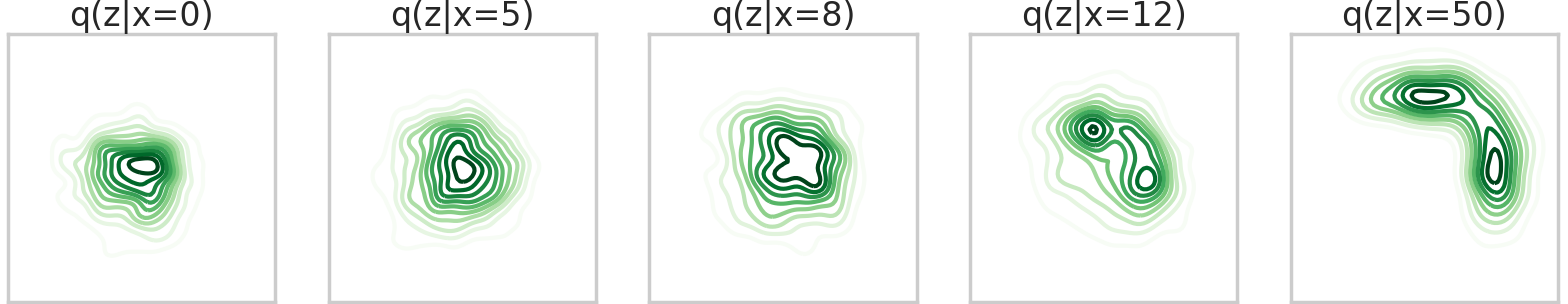
\includegraphics[width=\textwidth]{13288.png}
\caption{Average KL Divergence of 1.3288}
\end{subfigure}
}
\scalebox{0.8}{
\begin{subfigure}{\textwidth}
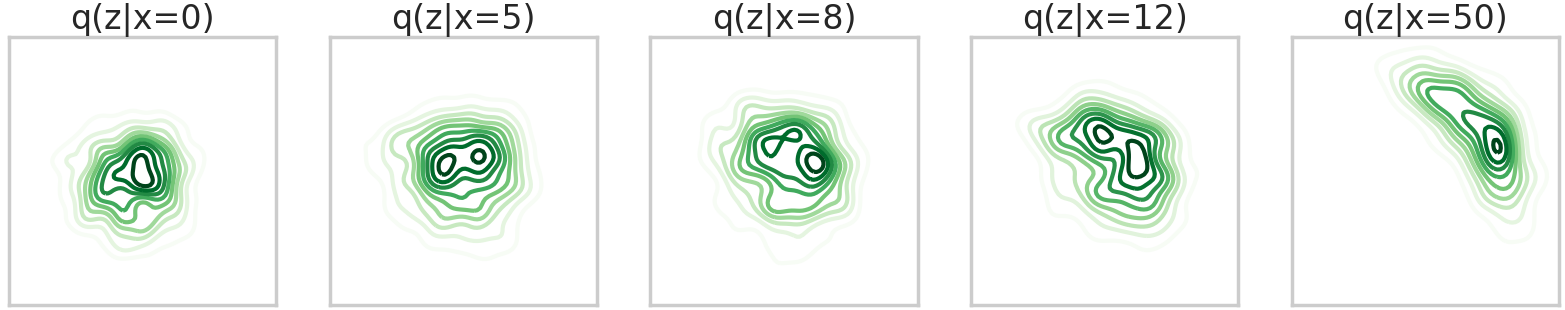
\includegraphics[width=\textwidth]{13963.png}
\caption{Average KL Divergence of 1.3963}
\end{subfigure}
}
\end{figure}
\end{frame}
\begin{frame}{Inference Experiment - Activation Function}{KL Divergence Plots}
\begin{figure}
\begin{subfigure}{0.49\textwidth}
\includegraphics[width=\linewidth]{truklmins/PCKLvsPCKLEXP.png}
\caption{Prior-Contrastive}
\end{subfigure}
\begin{subfigure}{0.49\textwidth}
\includegraphics[width=\linewidth]{truklmins/JCKLvsJCKLEXP.png}
\caption{Joint-Contrastive}
\end{subfigure}
\end{figure}
\begin{itemize}
\item Exponential output has smoother and faster convergence.
\end{itemize}
\end{frame}
\begin{frame}{Inference Experiment - Activation Function}{NELBOs}
\begin{figure}
\begin{subfigure}{0.49\textwidth}
\includegraphics[width=\linewidth]{nelbos/PCKLvsPCKLEXP.png}
\caption{Prior-Contrastive}
\end{subfigure}
\begin{subfigure}{0.49\textwidth}
\includegraphics[width=\linewidth]{nelbos/JCKLvsJCKLEXP.png}
\caption{Joint-Contrastive}
\end{subfigure}
\end{figure}
\begin{itemize}
\item More stable NELBO estimation by exponential output.
\item Variance of exponential output in joint-contrastive case increases over time.
\end{itemize}
\end{frame}
\section{Optimal Estimator Experiment}
\begin{frame}{Optimal Estimator Experiment}{Experiment Outline}
\begin{itemize}
\item Same inference problem as before.
\item Aim of this experiment is to verify that choice of estimator does not matter as long as it reaches equality.
\item Low training rate with high estimator to posterior optimisation ratio (100:1).
\item High posterior iterations.
\end{itemize}
\end{frame}
\begin{frame}{Optimal Estimator Experiment}{Results}
\begin{table}[h]
\scalebox{1.0}{
\begin{tabular}{|c|c|c|}
\hline
Algorithm & Mean KL Divergence & Standard Deviation\\
\hline
JC Reverse KL - $D_\alpha(z,x)$ & 1.3416 & 0.0068\\
\hline
JC Reverse KL - $r_\alpha(z,x)$ & 1.3397 & 0.0066\\
\hline
JC Reverse KL - $T_\alpha(z,x)$ & 1.3446 & 0.0108\\
\hline
JC GAN - $D_\alpha(z,x)$ & 1.3648 & 0.0242\\
\hline
JC GAN - $r_\alpha(z,x)$ & 1.3657 & 0.0302\\
\hline
JC GAN - $T_\alpha(z,x)$ & 1.3670 & 0.0387\\
\hline
\end{tabular}
}
\end{table}
\begin{itemize}
\item Prior-contrastive posteriors fully converged at $\approx 1.325$.
\item No significant difference in convergence between estimators in each f-divergence.
\item Reverse KL converged faster in joint-contrastive context.
\end{itemize}
\end{frame}
\begin{frame}{Optimal Estimator Experiment}{Joint-Contrastive KL Divergence Plots}
\begin{figure}
\begin{subfigure}{0.49\textwidth}
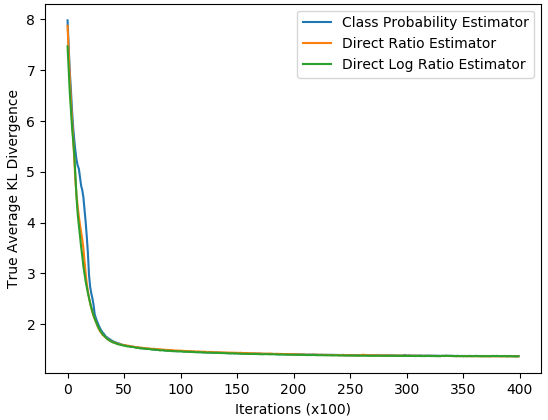
\includegraphics[width=\linewidth]{truklmins/JCADVvsJCADVexpvsJCADVgudlog.png}
\caption{GAN Divergence}
\end{subfigure}
\begin{subfigure}{0.49\textwidth}
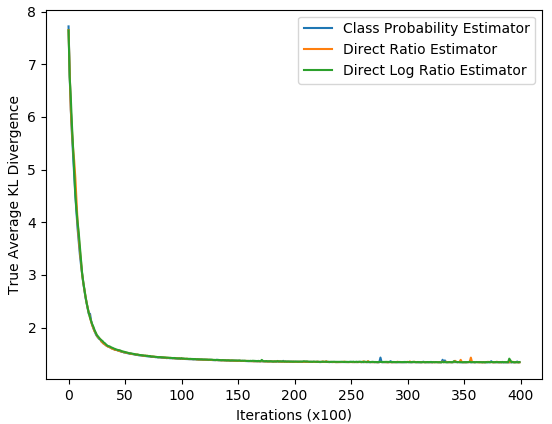
\includegraphics[width=\linewidth]{truklmins/JCKLDvsJCKLexpvsJCKLgudlog.png}
\caption{Reverse KL Divergence}
\end{subfigure}
\end{figure}
\begin{itemize}
\item Plots almost indistinguishable with exception of class probability estimator outlier in GAN divergence.
\end{itemize}
\end{frame}
\begin{frame}{Optimal Estimator Experiment}{Joint-Contrastive NELBO Plots}
\begin{figure}
\begin{subfigure}{0.49\textwidth}
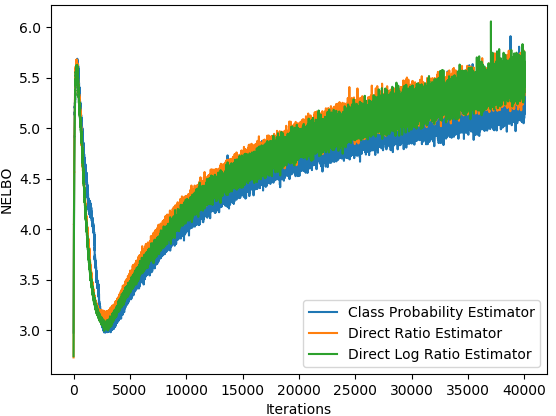
\includegraphics[width=\linewidth]{nelbos/JCADVvsJCADVexpvsJCADVgudlog.png}
\caption{GAN Divergence}
\end{subfigure}
\begin{subfigure}{0.49\textwidth}
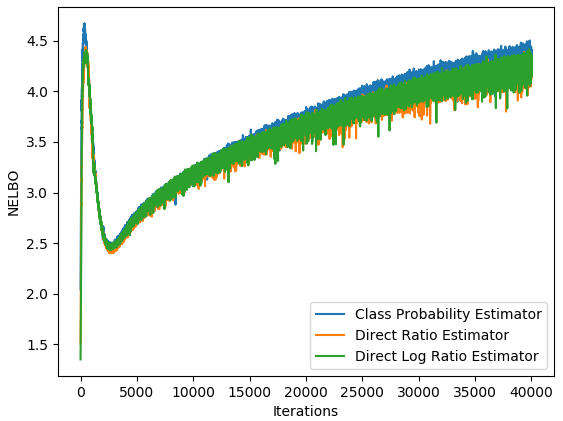
\includegraphics[width=\linewidth]{nelbos/JCKLDvsJCKLexpvsJCKLgudlog.png}
\caption{Reverse KL Divergence}
\end{subfigure}
\end{figure}
\begin{itemize}
\item Again very similar plots.
\item NELBO estimation smooth but has increasing variance over time.
\end{itemize}
\end{frame}
\section{Undertrained Estimator Experiment}
\begin{frame}{Undertrained Estimator Experiment}{Experiment Outline}
\begin{itemize}
\item Estimators are similar when they are optimal but what if they are not optimal?
\item Same inference experiment again.
\item Significantly reduce amount of estimator training between posterior iterations.
\item Increased posterior training rate.
\end{itemize}
\end{frame}
\begin{frame}{Undertrained Estimator Experiment}{Results}
\begin{table}[h]
\scalebox{0.8}{
\begin{tabular}{|c|c|c|}
\hline
Algorithm & Mean KL Divergence & Standard Deviation\\
\hline
JC Reverse KL - $D_\alpha(z,x)$ & 1.3786 & 0.0286\\
\hline
JC Reverse KL - $r_\alpha(z,x)$ & 1.3934 & 0.0410\\
\hline
JC Reverse KL - $T_\alpha(z,x)$ & 1.4133 & 0.0597\\
\hline
JC GAN - $D_\alpha(z,x)$ & 1.4017 & 0.0286\\
\hline
JC GAN - $r_\alpha(z,x)$ & 1.4086 & 0.0555\\
\hline
JC GAN - $T_\alpha(z,x)$ & 1.4214 & 0.0518\\
\hline
\end{tabular}
}
\end{table}
\begin{itemize}
\item Reverse KL divergence significantly better than GAN divergence.
\item $D_\alpha(z,x)<r_\alpha(z,x)<T_\alpha(z,x)$
\end{itemize}
\end{frame}
\begin{frame}{Undertrained Estimator Experiment}{Joint-Contrastive NELBO Plots}
\begin{figure}
\begin{subfigure}{0.49\textwidth}
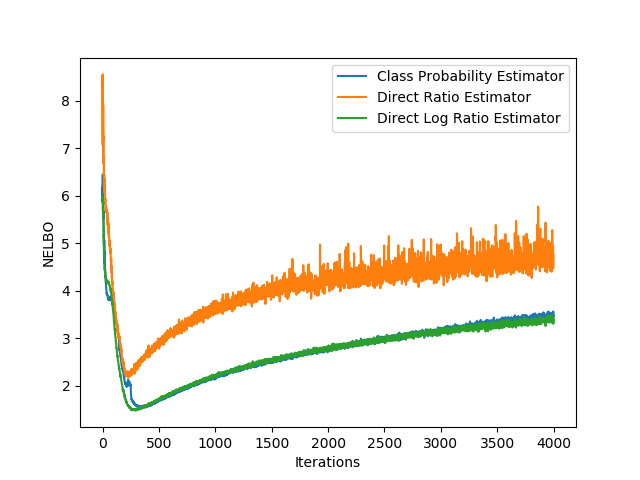
\includegraphics[width=\linewidth]{part2nelbos/JCADVvsJCADVexpvsJCADVgudlog.png}
\caption{GAN Divergence}
\end{subfigure}
\begin{subfigure}{0.49\textwidth}
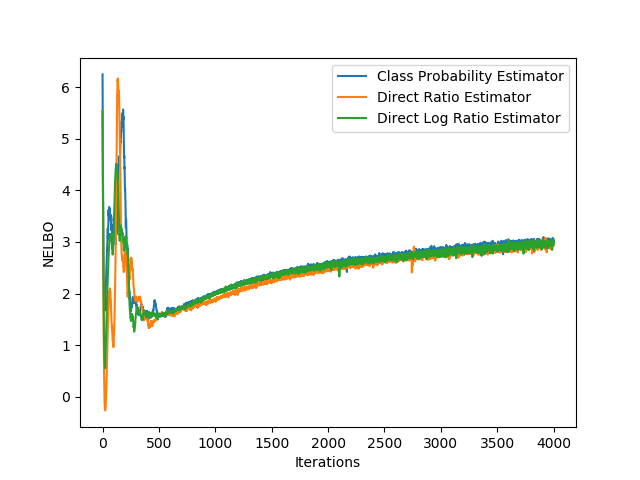
\includegraphics[width=\linewidth]{part2nelbos/JCKLDvsJCKLexpvsJCKLgudlog.png}
\caption{Reverse KL Divergence}
\end{subfigure}
\begin{itemize}
\item Unclear why direct ratio estimator has unusual NELBO plot: posterior convergence was not affected.
\end{itemize}
\end{figure}
\end{frame}
\subsection{Generation Experiment}
\begin{frame}{Generation Experiment}{Autoencoders}
\begin{itemize}
\item Likelihood $p_\theta(x|z)$ is now a neural network.
\item Posterior $q_\phi(z|x)$ represents data $x$ as lower dimensional latent $z$.
\item Likelihood $p_\theta(x|z)$ reconstructs data $\tilde{x}$ from $z$.
\item Generate new data $\tilde{x}$ using $z$ from $p(z)$.
\end{itemize}
\begin{figure}[h]
  \centering
  \scalebox{0.8}{
  \tikz{ %
    \node[latent] (x) {$\bm{x}$} ; %
    \node[det, right=of x] (q) {$q_\phi(z|x)$} ; %
    \node [latent, above=of x] (eps) {$\epsilon$} ;
    \node [latent, right=of q] (z) {$\bm{z}$} ;
    \node [det, right=of z] (p) {$p_\theta(x|z)$} ;
    \node [latent, right=of p] (pout) {$\tilde{\bm{x}}$} ;
    \edge {x} {q} ; %
    \edge {q} {z} ;
    \edge {eps} {q} ;
    \edge {z} {p} ;
    \edge {p} {pout} ;
  }
  }
\end{figure}
\[\min_{\theta, \phi} -\mathbb{E}_{q_\phi(z|x)q^*(x)}[\log p_\theta(x|z)]+\mathbb{E}_{q^*(x)}[KL(q_\phi(z|x)||p(z))]\]
\end{frame}
\begin{frame}{Generation Experiment}{Experiment Outline}
\begin{itemize}
\item MNIST dataset - $28\times 28$ grey-scale images of handwritten digits
\item Joint-contrastive context not tested here.
\item Again use undertrained estimator.
\item Use reconstruction error $\|x-\tilde{x}\|^2$ as metric.
\item Perform experiment with low dimensional latent space (2 dimensions) and high dimensional latent space (20 dimensions).
\item Low dimensional case had similar results to previous experiment.
\end{itemize}
\end{frame}
\begin{frame}{Generation Experiment}{Results - high dimensional latent space}
\begin{table}[h]
\scalebox{0.9}{
\begin{tabular}{|c|c|c|}
\hline
Algorithm & Mean Reconstruction Error & Standard Deviation\\
\hline
PC GAN - $D_\alpha(z,x)$ & 0.0444 & 0.0017\\
\hline
PC Reverse KL - $D_\alpha(z,x)$ & 0.0647 & 0.0019\\
\hline
\end{tabular}
}
\end{table}
\begin{itemize}
\item Direct ratio and direct log ratio estimators attempted to store numbers exceeding float64(max).
\item Exponential of $T_\alpha(z,x)$ taken in loss function.
\item $D_\alpha(z,x)$ ranges in $(0,1)$.
\item Value before sigmoid activation function for $D_\alpha(z,x)$ is log density ratio.
\item This time GAN divergence leads to better convergence than reverse KL.
\end{itemize}
\end{frame}
\begin{frame}{Generation Experiment}{Results - high dimensional latent space}
\begin{figure}
\begin{subfigure}{0.49\textwidth}
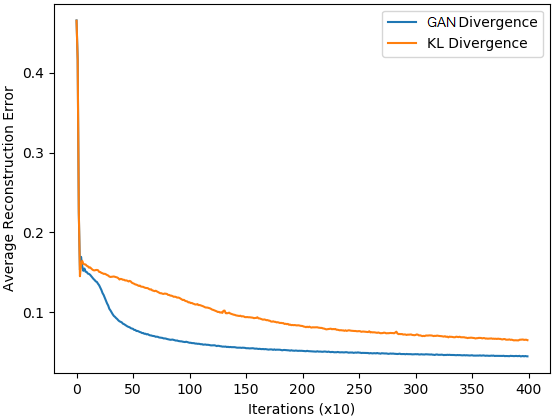
\includegraphics[width=\linewidth]{part4reconerrors/PCADVvsPCKLD.png}
\caption{Reconstruction Error}
\end{subfigure}
\begin{subfigure}{0.49\textwidth}
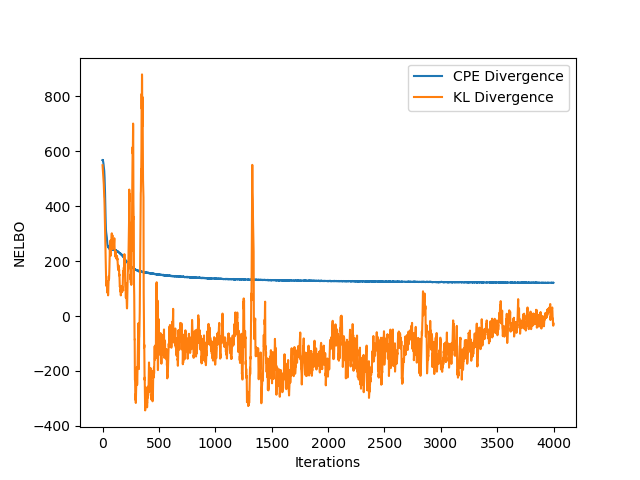
\includegraphics[width=\linewidth]{part4nelbos/PCADVvsPCKLD.png}
\caption{NELBO}
\end{subfigure}
\begin{itemize}
\item As before, GAN divergence is more stable.
\item Recall reverse KL divergence is initially unstable but stabilizes later.
\item In this case it fails to stabilise by the end of the program runtime.
\end{itemize}
\end{figure}

\end{frame}
%\begin{frame}{Blocks}
%\begin{block}{Block Title}
%You can also highlight sections of your presentation in a block, with it's own title
%\end{block}
%\begin{theorem}
%There are separate environments for theorems, examples, definitions and proofs.
%\end{theorem}
%\begin{example}
%Here is an example of an example block.
%\end{example}
%\end{frame}

% Placing a * after \section means it will not show in the
% outline or table of contents.
\section{Theory}
\begin{frame}{Theory}{Choice of f-divergence}
\begin{itemize}
\item Nowozin's f-GAN paper shows empirically that the reverse KL divergence is superior when it is additionally used to optimize the posterior.
\item Intuitive that the f-divergence used to optimize posterior is the best upper bound for estimator.
\end{itemize}
\end{frame}
\begin{frame}{Further Estimator Loss Function Analysis}{Estimator Parametrisation}
\begin{itemize}
\item $D_\alpha(u)$ has smallest bound of $(0,1)$, followed by $r_\alpha(u) \in \R^+$ and $T_\alpha(u)\in \R$.
\item The density ratio changes every time the posterior is optimised, and the estimator must catch up.
\item $D_\alpha(u)$ has a strictly lower displacement than $r_\alpha(u)$, that is, $|D_\alpha^{(n+1)}(u)-D_\alpha^{(n)}(u)|<|r_\alpha^{(n+1)}(u)-r_\alpha^{(n)}(u)|$.
\end{itemize}
\end{frame}


\section*{Summary}

\begin{frame}{Summary}
  \begin{itemize}
  \item
    The class probability estimator $D_\alpha(u)\simeq\frac{q(u)}{q(u)+p(u)}$ is the `best' parametrisation as it can store the\alert{highest density ratios}.
  \item
    Reverse KL divergence upper bound demonstrates \alert{initial instability} (especially when estimator is undertrained) but leads to \alert{faster convergence} when it stabilizes.
  \end{itemize}
  
  \begin{itemize}
  \item
    Outlook
    \begin{itemize}
    \item
      Still unclear exactly why reverse KL divergence is more unstable but more accurate when stable.
    \item
      Several more f-divergences exist which have unknown stability when undertrained.
    \end{itemize}
  \end{itemize}
\end{frame}



% All of the following is optional and typically not needed. 
%\appendix
%\section<presentation>*{\appendixname}
%\subsection<presentation>*{For Further Reading}
%
%\begin{frame}[allowframebreaks]
%  \frametitle<presentation>{For Further Reading}
%    
%  \begin{thebibliography}{10}
%    
%  \beamertemplatebookbibitems
%  % Start with overview books.
%
%  \bibitem{Author1990}
%    A.~Author.
%    \newblock {\em Handbook of Everything}.
%    \newblock Some Press, 1990.
% 
%    
%  \beamertemplatearticlebibitems
%  % Followed by interesting articles. Keep the list short. 
%
%  \bibitem{Someone2000}
%    S.~Someone.
%    \newblock On this and that.
%    \newblock {\em Journal of This and That}, 2(1):50--100,
%    2000.
%  \end{thebibliography}
%\end{frame}

\end{document}


